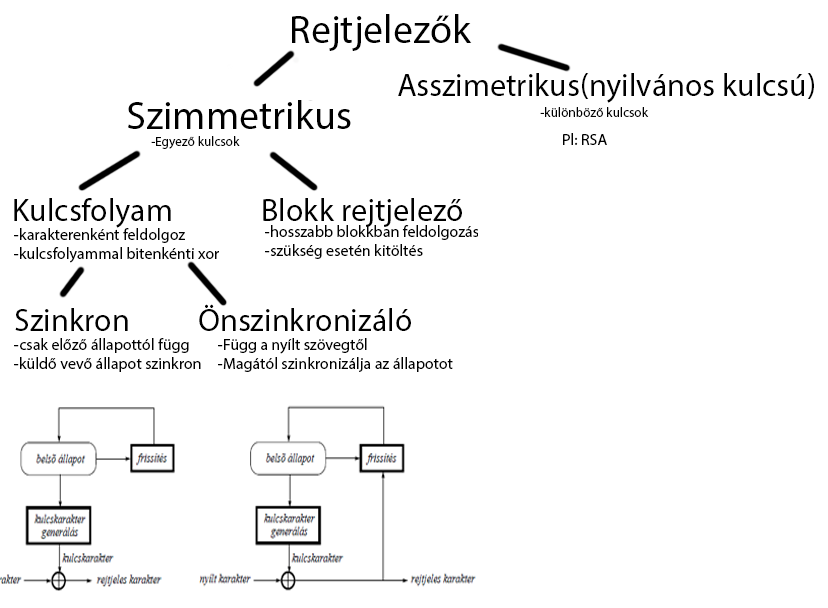
\includegraphics[scale=0.85]{img/Typessmall}

\section{Szimmetrikus kulcsu Rejtjelezés}
(1. dia)
\subsection{Betűnkénti lineáris rejtjelező}
	M = (26 betus angol abc) = (abcdefghijklmnopqrstuvwxyz)\\[2pt]
	C = M $\leftarrow$ kodszavak\\[2pt]
	$c = a \cdot m + b \ mod \ 26 $ \small(m = bemeneti szoveg) \normalsize
	\begin{enumerate}
		\item Adjuk meg a dekódoló transzformációt! Milyen megszorítást kell tenni "a" kulcselemre?
		\item Sikerult két nyílt szöveg - rejtett szöveg párt megismerni:\\[2pt] $m_1 = 4,\ c_1 = 14; \quad m_2 = 10,\ c_2 = 10, \quad $ Hatarozzuk meg a kulcsot!
	\end{enumerate}

\subsection{Lineáris blokk rejtjelező}

	$\underline{y} = \underline{\underline{A}}\, \underline{x}+\underline{b}$ \quad - A nxn es \textit{bináris} mátrix, x,y,b n hosszú bináris oszlopvektorok

	\small \textit{M: Nem szokták használni }\normalsize

\subsection{One time pad} %TODO Valahogy kiemelni ezt a blokkot mint zsolti
	\begin{definicio}{Mézga Géza} \textbf{Tökéletes rejtjelező} \small (perfect encryption) \normalsize \\[2pt]
	Ha a nyílt szöveg valószínűségi változó statisztikailag független a rejtett szöveg valószínűségi változótól $\Longrightarrow$ rejtjeles szöveget legallgató támadó tetszőleges erőforrás mellett sem képes a nyílt szövegre jobb döntést hozni, mint amire a megfigyelést megelőzően képes ( ugyan annyi "a" a bemeneten mint kimeneten stb.)\\[2pt]
\end{definicio}

PL: $y := x + k \ mod\ 2$\\[2pt]
x = 01001101 01011101\\[2pt]
k = 11010000 11101011 \quad $\leftarrow$ \textit{ez a lenyeg, mindig mással van összeadva} \\[2pt]
	\forceindent \forceindent \forceindent	$\Downarrow$\\[2pt]
y = 10011101 10110110\\[2pt]

PL2: $y := x + k \ mod\ 26$

x= ONETIMEPAD \\[2pt]
k= TBFRGFARFM \\[2pt]
\forceindent \forceindent \forceindent	$\Downarrow$\\[2pt]
y= IPKLPSFHGQ \\[2pt]
O + T mod 26 = I , N + B mod 26 = P , E + F mod 26 = K $ \ldots$\\[2pt]
\small \textit{Megtobb pelda dian hasznosak} \normalsize

\subsection{Shamir háromlépéses protokollja:}

\subsection{}
